\documentclass{article}
\usepackage{amsmath}
\usepackage{amssymb}
\usepackage{fancyhdr}
\usepackage[utf8]{inputenc}
\usepackage{tcolorbox}
\usepackage[left=1in, right=1in, top=1.5in, bottom=1in]{geometry}
\usepackage{tikz}
\usepackage{enumerate}
\usepackage{enumitem}
\usepackage{array}

\pagestyle{fancy}
\fancyhf{} % Clear all header and footer fields
\fancyhead[L]{Your Name:} % Left header with name
\fancyhead[R]{September 30th 2025} % Right header with date
\renewcommand{\headrulewidth}{0.4pt} % Horizontal line below the header

\begin{document}

% Main title
\begin{center}
    \Large \textbf{Math 115E Class} \\
    \vspace{0.2cm}
    \normalsize Midterm Class Review \\
\end{center}

\section*{Activity 1}

State the interval notation in both forms
\\\\
\noindent % Prevents initial paragraph indentation
\noindent % Ensures alignment to the left margin
\begin{minipage}{0.45\textwidth}
    \centering
    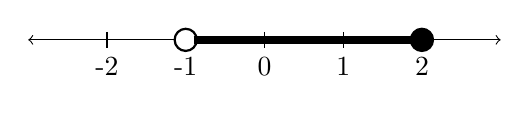
\begin{tikzpicture} % TOP LEFT PLOT: (-1, 2]
        % Draw the number line
        \draw[<->] (-3,0) -- (3,0);
        \foreach \x in {-2,-1,0,1,2}
        \draw (\x, 0.1) -- (\x, -0.1) node[below] {\x};

        % Draw the open circle at -1
        \draw[fill=white, thick] (-1,0) circle (4pt);
        % Draw the closed circle at 2
        \draw[fill=black, thick] (2,0) circle (4pt);

        % Draw the line segment between the two points
        \draw[black, line width=3pt] (-0.9,0) -- (2,0);
    \end{tikzpicture}
    
    \vspace{2cm} % <<< ADDED VERTICAL SPACE HERE
    
    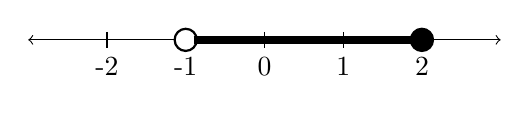
\begin{tikzpicture} % BOTTOM LEFT PLOT: (-1, 2] (Duplicate from original)
        % Draw the number line
        \draw[<->] (-3,0) -- (3,0);
        \foreach \x in {-2,-1,0,1,2}
        \draw (\x, 0.1) -- (\x, -0.1) node[below] {\x};

        % Draw the open circle at -1
        \draw[fill=white, thick] (-1,0) circle (4pt);
        % Draw the closed circle at 2
        \draw[fill=black, thick] (2,0) circle (4pt);

        % Draw the line segment between the two points
        \draw[black, line width=3pt] (-0.9,0) -- (2,0);
    \end{tikzpicture}
\end{minipage}% 
\hfill
\begin{minipage}{0.45\textwidth}
    \centering
    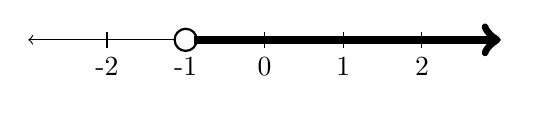
\begin{tikzpicture} % TOP RIGHT PLOT: (-1, \infty)
            % Draw the number line
            \draw[<->] (-3,0) -- (3,0);
            \foreach \x in {-2,-1,0,1,2}
            \draw (\x, 0.1) -- (\x, -0.1) node[below] {\x};

            % Draw the open circle at -1
            \draw[fill=white, thick] (-1,0) circle (4pt);

            % Draw the line segment between the two points
            \draw[black, line width=3pt, ->] (-0.9,0) -- (3,0);        
    \end{tikzpicture}
    
    \vspace{2cm} % <<< ADDED VERTICAL SPACE HERE
    
    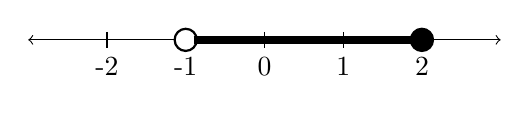
\begin{tikzpicture} % BOTTOM RIGHT PLOT: (-1, 2] (Duplicate from original)
        % Draw the number line
        \draw[<->] (-3,0) -- (3,0);
        \foreach \x in {-2,-1,0,1,2}
        \draw (\x, 0.1) -- (\x, -0.1) node[below] {\x};

        % Draw the open circle at -1
        \draw[fill=white, thick] (-1,0) circle (4pt);
        % Draw the closed circle at 2
        \draw[fill=black, thick] (2,0) circle (4pt);

        % Draw the line segment between the two points
        \draw[black, line width=3pt] (-0.9,0) -- (2,0);
    \end{tikzpicture}
\end{minipage}
\vspace{1.2cm}
\section*{Activity 2/3}
\noindent
\begin{minipage}[c]{0.45\textwidth}
    
    What is the domain and range for plots:
    \begin{enumerate}
    \item Graph (E)
    \vspace{3cm}
    \item Graph (F)
    \vspace{3cm}
    \item Graph (G)
    \vspace{3cm}
    \item Graph (H)
\end{enumerate}
\end{minipage}%
\hfill
\begin{minipage}[c]{0.50\textwidth} % Minipage for the TikZ graph (increased width slightly for labels)
    \centering % Center the TikZ picture within its minipage
    
    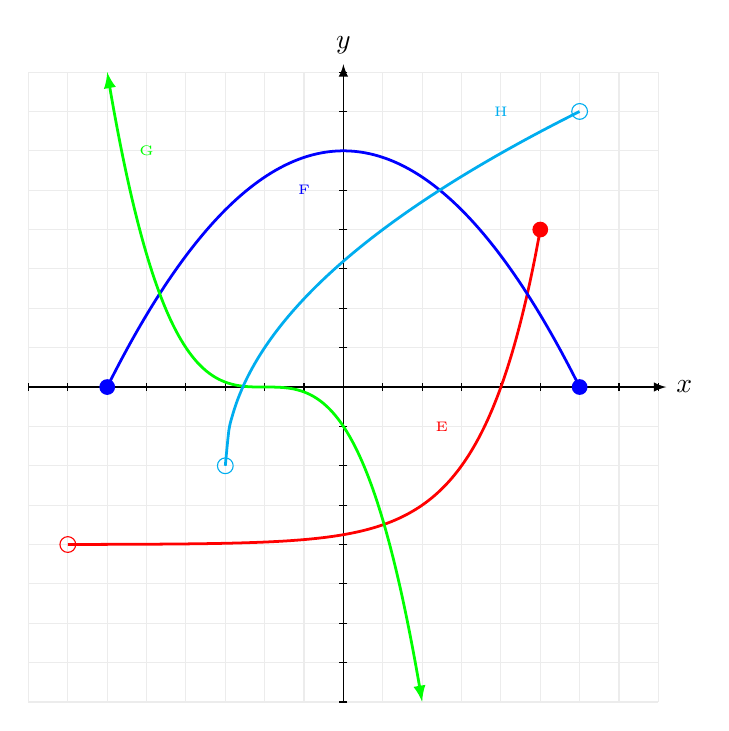
\begin{tikzpicture}[scale=0.50]
        \draw[gray!15,step=1cm] (-8,-8) grid (8,8);
        \draw[line width=0.2mm, -latex] (-8,0) -- (8.2,0) node[right] {$x$};
        % The \foreach loop for x-axis numbers has been modified
        \foreach \x in {-8,...,8} \draw (\x,.1)--(\x,-.1);
        \draw[line width=0.2mm,  -latex] (0,-8) -- (0,8.2) node[above] {$y$};
        % The \foreach loop for y-axis numbers has been modified
        \foreach \y in {-8,...,8} \draw (.1,\y)--(-.1,\y);

        % Red line with adjusted label 'E'
        \draw[red,line width=1pt] plot[smooth, samples=100, domain= -7:5] (\x,{2^(\x-2) - 4}) node[font=\tiny] at (2.5, -1) {E};
        \draw[red] (-7, -4) circle (0.2);
        \fill[red] (5, 4) circle (0.2);
        % Blue line with adjusted label 'F'
        \draw[blue,line width=1pt] plot[smooth, samples=100, domain= -6:6] (\x,{-1/6*(\x-6)*(\x+6)}) node[font=\tiny] at (-1, 5) {F};
        \fill[blue] (-6, 0) circle (0.2);
        \fill[blue] (6, 0) circle (0.2);
        % Green line with adjusted label 'G'
        \draw[green,line width=1pt, latex-latex] plot[smooth, samples=100, domain= -6:2] (\x,{-1/8*(\x+2)^3}) node[font=\tiny] at (-5, 6) {G};
        % Cyan line with adjusted label 'H'
        \draw[cyan,line width=1pt] plot[smooth, samples=100, domain= -3:6] (\x,{3*sqrt(\x+3) - 2}) node[font=\tiny] at (4, 7) {H};
        \draw[cyan] (-3, -2) circle (0.2);
        \draw[cyan] (6, 7) circle (0.2);
    \end{tikzpicture}

\end{minipage}
\vspace{1cm}
\noindent
\section*{Activity 4}
Simplify or expand the Following:\\
\begin{minipage}[t]{0.45\textwidth}
    \begin{enumerate}
        \item $(a+b)^2$
        \\\\\\\\
        \item $(-2)^2 + (-3)$
        \\\\\\\\
        \item $x^2 \cdot x^3 \cdot x$ 
    \end{enumerate}
\end{minipage}%
\hfill
\begin{minipage}[t]{0.45\textwidth}
    \begin{enumerate}
        \setcounter{enumi}{4} % continues numbering
        \item $2(-3)(-1)(-x)$
        \\\\\\\\
        \item $ 10x + 50x - 70x$
        \\\\\\\\
        \item $(x-2)(3x+1)$

    \end{enumerate}
\end{minipage}
\vspace{3cm}
\section*{Activity 5}
Simplify or expand the Following:\\
\begin{minipage}[t]{0.45\textwidth}
    \begin{enumerate}
        \item $f(x) = 2x - 10, f(6)=?$
        \\\\\\\\\\
        \item $f(x) = 10 - 5x, f(-1)=?$
        \\\\\\\\\\
        \item $f(x) = -x^2 + 4, f(4)=?$
    \end{enumerate}
\end{minipage}%
\hfill
\begin{minipage}[t]{0.45\textwidth}
    \begin{enumerate}
        \setcounter{enumi}{4} % continues numbering
        \item $f(x) = 2 - x, f(x+3)=?$
        \\\\\\\\\\
        \item $f(x) = x^2 + x + 1, f(3x)=?$
        \\\\\\\\\\
        \item $f(x)= x^2 - 1, f(x+3)=?$

    \end{enumerate}
\end{minipage}
\vspace{4cm}

\section*{Activity 6}
Given two functions: $f(x) = 2x+1$ and $g(x) = x^2 - 1$
\\
\begin{minipage}[t]{0.45\textwidth}
    \begin{enumerate}
        \item Find $(f \circ g)(x)$
        \\\\\\\\
        \item Find $(g \circ f)(x)$
        \\\\\\\\
        \item Find $(f + g)(x)$
    \end{enumerate}
\end{minipage}%
\hfill
\begin{minipage}[t]{0.45\textwidth}
    \begin{enumerate}
        \setcounter{enumi}{4} % continues numbering
        \item Find $(f - g)(4)$
        \\\\\\\\
        \item Find $(f \cdot g)(x)$
        \\\\\\\\
        \item Find $(f \circ f)(6)$

    \end{enumerate}
\end{minipage}
\vspace{2cm}
\section*{Activity 7}
\noindent
\begin{minipage}[c]{0.60\textwidth}
    \begin{enumerate}
        \vspace{0.5cm}
        \item Let $f(x)$ be the function given by the graph \\
              Let $g(x)$ be given as $g(x)=1-x-x^2$ \\
              Let $h(x)$ be the function given by the table
              \begin{center}
                \raggedright
                \begin{tabular}{|c||c|c|c|c|c|c|c|c|}
                    \hline
                    $x$ & -5 & -3 & -1 & 0 & 2 & 4 & 5 & 6 \\
                    \hline
                    $h(x)$ & -2 & -0.5 & 0.5 & 2 & 3 & 9 & 0 & 15 \\
                    \hline
                \end{tabular}
        \end{center}
              Find the following
              \begin{enumerate}
                \item Find $g(f(3))$
                \vspace{1.2cm}
                \item Find $(f \cdot g)(2)$
                \vspace{1.2cm}
                \item Find $h(g(2))$
                \vspace{1.2cm}
                \item Find $h(f(-1))$
                \vspace{1.2cm}
                
              \end{enumerate}
        \end{enumerate}
\end{minipage}%
\hfill
\begin{minipage}[c]{0.40\textwidth} % Minipage for the TikZ graph (increased width slightly for labels)
    \centering % Center the TikZ picture within its minipage
    \vspace{-4cm}
    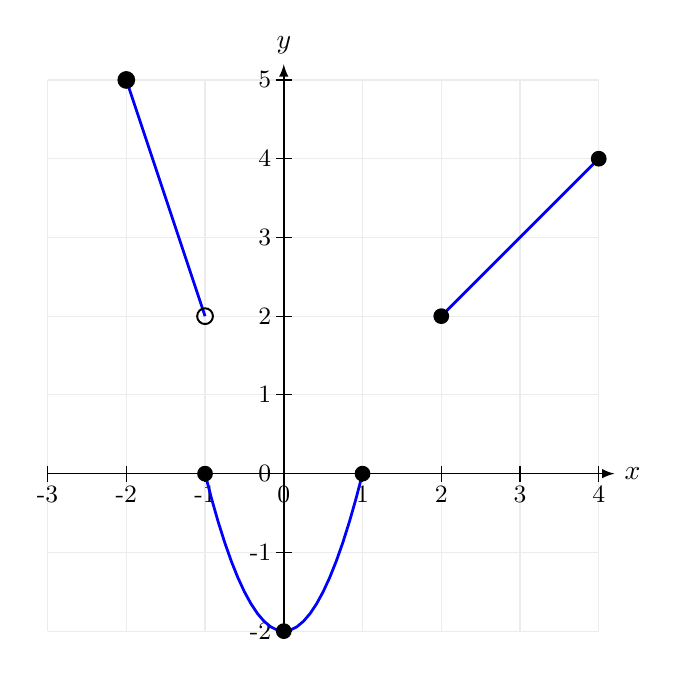
\begin{tikzpicture}[scale=1]
    \draw[gray!15,step=1cm] (-3,-2) grid (4,5);
    \draw[line width=0.2mm, -latex] (-3,0) -- (4.2,0) node[right] {$x$};
    \foreach \x in {-3,...,4} \draw (\x,.1)--(\x,-.1) node[below=1pt, font=\small] at (\x,0) {\x};
    \draw[line width=0.2mm,  -latex] (0,-2) -- (0,5.2) node[above] {$y$};
    \foreach \y in {-2,...,5} \draw (.1,\y)--(-.1,\y) node[left=1pt, font=\small] at (0,\y) {\y};

    % Slightly curved line from (-2,5) to (-1,2)
    \draw[blue, line width=1pt, smooth] plot coordinates {(-2, 5) (-1, 2)};
    \draw[fill=white, black, line width=0.25mm] (-2, 5) circle (0.1);
    \draw[black, line width=0.25mm] (-1, 2) circle (0.1);

    % Parabola from (-1,0) to (1,0) with vertex (0,-2)
    \draw[blue, line width=1pt] plot[domain=-1:1] (\x,{2*\x*\x - 2});
    \fill[black] (-1, 0) circle (0.1);
    \fill[black] (0, -2) circle (0.1);
    \fill[black] (1, 0) circle (0.1);

    % Straight line from (2,2) to (4,4)
    \draw[blue, line width=1pt] plot[domain=2:4] (\x, \x);
    \fill[black] (2, 2) circle (0.1);
    \fill[black] (4, 4) circle (0.1);

\end{tikzpicture}
    
    
\end{minipage}
\end{document}